
\chapter{Description of our prototype for spatio-angular illumination}
\label{sec:dev1}
\begin{summary}
  In the preceding chapter I showed the underlying concept of our
  spatio-angular microscope. Here I discuss additional details that
  are important for the practical implementation.

  I explain the beam path, electronic synchronization of the displays
  with other components and an algorithm to transform the coordinate
  system of the camera pixels into the coordinate system of the focal
  plane SLM.
  
  The pupil plane SLM was specifically developed for our project by    
  our partner Fraunhofer IPMS (Dresden, DE). 
\end{summary}
\section{Description of the optical components}
In the preceding chapter I have shown the beam path for
transmissive displays (in \figref{fig:memi-simple}). Such SLM have a
very low transmission in practice. Therefore we use reflective
displays in our prototype.

In \figref{fig:memi-real} I adjusted the beam path accordingly. This
schematic also depicts the optics we use to adapt light from the laser
to fill the etendue of our system. The light source enters the system
from the bottom left. The optic components are color corrected and
have anti-reflex coating for wavelengths in the range from
\unit[400]{nm} to \unit[700]{nm}.

The system successively illuminates the pupil plane SLM --- a greyscale
micro mirror array developed by our project partner Fraunhofer IPMS
Dresden --- and the focal plane SLM, a commercial binary liquid crystal
on silicon display. \nomenclature{DBS}{Dichromatic beam splitter}

\begin{figure}[!htbp]
  \centering
  \svginput{2}{memi-real}
  \caption{Schematic of the light path through our microscope. Laser
    light enters from the lower left, is scrambled and homogenized to
    illuminate the pupil plane SLM in $\textrm{P}''$ and the focal
    plane SLM in $F'$. $F$ is the field plane in the sample and its
    primed versions are conjugated planes. $P$ is the pupil of the
    objective. Field mask $B_0$ and Fourier stop $B_1$ are adjustable
    circular apertures. PBS is a polarizing beam splitter. DBS is a
    dichromatic beam splitter.  The red boxes deliminate subsystems of
    the illumination system: {\color{Orchid}\bf A$_1$ and A$_2$:}
    light scrambling and homogenization, {\color{Orchid}\bf B:}
    Fourier-optical filter to provide intensity modulating pupil plane
    SLM. {\color{Orchid}\bf C:} Polarization based intensity modulator
    as focal plane SLM. {\color{Orchid}\bf D:} Wide-field fluorescence
    microscope with detection path.}
  \label{fig:memi-real}
\end{figure}

\subsection{Ensuring homogeneous illumination}
A quantitative evaluation of our experiments (section
\ref{sec:results}) with different illumination patterns is simplified
when both pupil plane SLM and focal plane SLM are uniformly
illuminated.  Below we discuss an optical setup that attains
homogeneity of the illumination of both displays.

We use either a laser\footnote{Lasever LSR473H, diode-pumped solid
  state laser, output power 600mW, $\lambda=\unit[473]{nm}$} or a
light emitting diode (LED) as the light source in our experiments. The
LED\footnote{Huey Jann HPB8-48KBD, wavelength $\unit[(463\pm1)]{nm}$,
  brightness \unit[35]{lm}, view angle
  $120{}^\circ$ %, FIXME TODO: Flaeche messen
} we use has a large active area.  Due to etendue mismatch a
relatively large amount of light will never reach the sample. However,
it is easy to achieve a homogeneous illumination with an
LED. Moreover, the LED can be quickly switched on and off
electronically. Nevertheless, it would be better to use an LED with a
smaller active area but those are hard to find.
% source code: https://github.com/plops/ledtlc/blob/master/ledtlc.ino

 % \footnote{The DPSS Laser doesn't allow fast
 %  direct electronic switching at full power. We have to use an
 %  acousto-optic modulator connected with the additional expense of its
 %  optical alignment (FIXME siehe spaetere ref section).}.

Unlike an LED, a laser delivers light of considerably higher spectral
radiance ($\unit[]{W/(sr\, m^2 nm)}$). Thus it is in principle possible
to use the laser as a highly efficient light source for our
system. Unfortunately, the high spectral and spatial coherence of a
laser often leads to high-contrast fluctuations of the irradiance and
we have to compensate for this by time averaging.

When using the laser, we send its collimated Gaussian beam into a
bundle\footnote{Fiber bundle with circular cross-section (Loptek,
  Berlin, DE), \unit[1.1]{mm} diameter and \unit[2]{m} length. The
  beam broadening is $3{}^\circ$ and increases, when the bundle is
  bent \citep{Ipp2009}.}  of randomly distributed fibers. This
randomizes the light distribution at the bundle output and also
broadens the illumination angles.

A relay system (A$_1$ in \figref{fig:memi-real}) images the circular
output of the fiber bundle onto the entrance of a light pipe. This
relay system contains a rotating microlens array\footnote{Array of
  cross-oriented cylindrical lenses on both sides with a pitch of
  \unit[0.5]{mm} resulting in an effective focal length of
  \unit[6.9]{mm} (LIMO, Dortmund, DE).}. It is driven by a motor with
the axis of rotation displaced from the optical axis. Integrating
sufficiently long over the time-variations in the intensity pattern
allows reduction of speckle.

Both the fiber bundle and microlens array increase the etendue of the
laser illumination to the optimum value, which is given by one of our
SLM as discussed on page \pageref{sec:etendue-mma}.

The integration tunnel shown in \figref{fig:integrator-rod} is hollow
and has a quadratic cross-section. The mixing effect of the tunnel can
be understood by considering the irradiance in the plane of the tunnel
output as it would occur without tunnel.  Drawing the outline of the
square cross-section into this irradiance map selects the light that
reaches this plane directly without any reflection.  Surrounding this
outline with four identical copies that touch its edges selects the
light that will reach the output plane after one reflection. The
irradiance maps from neighbouring squares are mirrored and added to
the direct illumination. Depending on the numerical aperture of the
input light, more reflections may occur --- resulting in the addition
of irradiance from next-nearest-neighbours.

This integration tunnel improves the uniformity of the light
distribution in the output plane without altering the numerical
aperture of the light.  The more subregions are superimposed, the
better will be the uniformity of the illumination.  Assuming $N$
subregions were overlaid and their contributions were statistically
independent, then according to the central limit theorem the standard
deviation of the irradiance is proportional to $1/\sqrt{N}$
\citep{Koshel2012}.
We also align the source distribution to be rotationally symmetric
about the optical axis and obtain an even more uniform output because
positive and negative slopes from different subregions compensate in
the superposition.

The dimensionis of the integration tunnel in our sytem is
$\unit[2.5]{mm}\times\unit[2.5]{mm}\times\unit[250]{mm}$ and ensures
enough reflections for homogeneous illumination. A relay system
magnifies the tunnel output to $\unit[4]{mm}\times\unit[4]{mm}$ in the
plane $\textrm{F}'''$.

\jpginput{8cm}{integrator-rod}{Hollow mirror-integrator tunnel with a
  quadratic cross section of \unit[2.5]{mm} side length and
  \unit[250]{mm} length.}


During the planning phase we also considered a homogenization design
based on a fly's eye condensor (two consecutive microlens
arrays). According to simulations performed by In-Vision, this,
however, would have been more difficult to adjust than the tunnel. In
particular the system would have been more dependent on illumination
wavelength compared to the tunnel.

In summary the following points are important in order to achieve
homogeneous illumination of focal and pupil plane with the tunnel:
%\renewcommand{\labelitemi}{$\star$}
\begin{itemize}
\item The image of the end of the bundle should properly cover the
  tunnel entrance. Especially the corners of the tunnel should not be
  darker than the center. Inhomogeneous illumination at the tunnel
  entrance leads to inhomogeneous illumination of the pupil plane SLM.
\item The end of the fibre bundle must be adjusted in four axes
  (centering and angle).
\item The focal length of the microlenses should be chosen shorter
  than predicted by pure etendue calculation in order to compensate
  coating defects on the edges of the cemented glass mirrors.
\end{itemize}

\subsection{Fourier optical filter for contrast generation on pupil
  plane SLM}
\label{sec:mma}
The micro mirror array consists of
torsion mirrors that modulate the phase of the light (see
\figref{fig:mma} for images of the device). It is used as a pupil plane SLM.
In order to modulate the
intensity we use the Fourier optical filter denoted as
'schlierenoptics' in \figref{fig:memi-real}~B.

The device itself is documented in more detail in the following
references: design of the actuators \citep{Schmidt2010}, grey value
images and contrast measurement \citep{Berndt2010} and per-pixel
calibration of the deflection angle using a white light interferometer
\citep{Berndt2011,Berndt2007}.

\jpginput{14cm}{mma}{{\bf left:} Scanning electron microscope image of
  the micro-mirror array (MMA).  The pixel pitch of the device is
  \unit[0.016]{mm}. The hinges for the tilt movement and the
  electrodes are clearly visible. {\bf middle:} Optical reflective
  microscope image of the MMA. {\bf right:} Rendering of how a 8x8
  checker board pattern would be displayed on the device. The
  deflection angles are exaggerated.  Electron and optical micrograph
  by Fraunhofer IPMS Dresden, Germany}

The lens L1 has two purposes: First, it images the field mask B0 into 
the Fourier stop B1. Second, the plane $\textrm{P}''$ with the phase
SLM is imaged to infinity.

With undeflected micro mirrors, the SLM has no signifcant effect and
works like a plane mirror. Both planes $\textrm{F}''$ and
$\textrm{P}'$ are then homogeneously illuminated.

If the left half of the micro mirrors are tilted, then they direct the
light along the dashed line in \figref{fig:memi-real}. This light is
absorbed by the field stop B1 and therefore missing in $\textrm{P}'$,
i.e.\ the right side in $\textrm{P}'$ is dark. The total radiant flux
($\unit[]{W}$) through the beam stop in $\textrm{F}''$ decreases while
the transmitted irradiance ($\unit[]{W/m^2}$) remains homogeneous.

Since the torsion angles of the micro mirrors are quite small, the
contrast generation in our Fourier filtering device (denoted as
schlierenoptics in \figref{fig:memi-real}) is somewhat complicated. In
the following I will describe the effect of the MMA phase function on
a plane monochromatic wave. In particular, I will investigate the
amount of light in the zeroth diffraction order depending on the
torsion angle. Furthermore, the structure of the diffraction image
limits the maximum acceptance angle of the system. I will show, that
the acceptance angle is just barely sufficient for our experiments.

To describe the Fourier pattern, I first consider a single pixel with
index $p$ and width $w=\unit[16]{\mu m}$. In one dimension its shape
can be described by the following equation:
\begin{align}
  T_p(x)=\delta(x-x_p)\otimes\left(\rect(x/w)\cdot e^{i k_{px} x}\right)\quad\textrm{with}\ \rect(x):=\begin{cases} 1 & |x|<1/2 \\ 0 & \textrm{else} \end{cases} \label{eq:tp}
\end{align}
The convolution with the $\delta-$distribution shifts the pixel to the
position $x_p$ and $k_{px}$ describes the torsion angle of the $p-$th
mirror.  With the Fourier transform 
\begin{align}
  \frac{1}{w}\int_{-w/2}^{w/2} e^{ikx} \textrm{d}x =
  \frac{\sin(kw/2)}{kw/2} =: \sinc(kw/2)
\end{align}
one can express the Fraunhofer diffraction image of a single pixel:
\begin{align}
  \widetilde T_p(k_x) = e^{ik_x x_p} \left(w \sinc(kw/2)\otimes\delta(k_x-k_{px})\right)
  = e^{ik_x x_p} w \sinc\left((k+k_{px})\cdot w/2\right)
\end{align}
That is, the sinc-shaped diffraction image of the pixel shifts in
k-space depending on the deflection of the mirror.  Now I will derive
the relationship between the direction of the reflected phase front,
described by $k_{px}$, and the deflection $l$ of the mirrors from the
equilibrium position. For that I consider the term $e^{i k_{px} x}$ in
equation (\ref{eq:tp}) at the point $x=-w/2$. The distance $l$ is
traversed twice during the reflection (see
\figref{fig:diffraction}~left). This can be expressed in the following
equation.
\begin{align}
  e^{-ik_{px} \frac{w}{2}} = e^{\frac{2\pi i}{\lambda} 2l} 
\end{align}
Solving for $k_{px}$ results in:
\begin{align}
  k_{px} &= -\frac{2\pi}{\lambda} \frac{4l}{w}
\end{align}



\begin{figure}[htbp]
  \centering 
  \svginput{1}{deflection-kp}
  \quad\quad\quad\quad
  \svginput{1}{diffraction-orders}
  \caption{{\bf left:} Schematic indicating the deflection $l$ of a
    micro mirror. {\bf right:} Illustration of diffraction orders of
    the micro mirror array.}
  \label{fig:diffraction}
\end{figure}
Now I \cma{1D diffraction problem} investigate a line of $N$ pixels in
the plane $P''$ in \figref{fig:memi-real}. The $N$ pixels are
distributed with a pitch of $\Lambda$, i.e.\ the $p-$th pixel is
centered at $x_p=\Lambda\cdot p$ with the index $p=-\lfloor
N/2\rfloor,\dots,\lfloor N/2\rfloor+1$ where $\lfloor N/2\rfloor$
denotes the biggest integer below $N/2$. For simplicity I neglect gaps
between the mirrors and the surface deformations at the central
attachment point (see \figref{fig:mma}).  Therefore, in the following
derivations I consider the pixel pitch to be identical with the pixel
width: $\Lambda=w=\unit[16]{\mu m}$.  The Fourier spectrum $\widetilde
T_\textrm{line}$ of a line of $N$ pixels is (positioned in the plane
$F''$ in \figref{fig:memi-real}):
\begin{align}
  \widetilde T_\textrm{line}(k_x) & = \sum_{p=-\lfloor N/2\rfloor}^{\lfloor N/2\rfloor+1} T_p(k_x) 
  = w \sum_{p=-\lfloor N/2\rfloor}^{\lfloor N/2\rfloor+1} e^{ik_x \Lambda p} \sinc\left(\frac{w}{2}(k_x+k_{px})\right) \label{eq:tline}
\end{align}

The sum over the first exponential term in this expression corresponds
to a grating of $N$ lines with a period equal to the pixel
pitch. Depending on the torsion angle of individual mirrors the terms
are modulated with a correspondingly shifted sinc-function.  In the
first diagram in \figref{fig:maxima-diffraction}~left the intensity
$|\sum_p \exp(ik_x \Lambda p)|^2$ of the sum over the phase factor is
displayed for $N=1$, $N=4$ and $N=20$. With an increasing number of
mirrors $N$ the diffraction peaks become more pronounced. The micro
mirror device that was built for our prototype has $N=256$, that is to
say the sum over the phase factors corresponds to a train of fine
diffraction orders at wave vectors $k_x^{(m)}$ described by the
grating equation (see \figref{fig:diffraction}~right):
\begin{align}
  \sin\theta = \frac{m \lambda}{\Lambda}, \qquad k_x^{(m)} =
  \frac{2\pi}{\lambda} \sin\theta = m \frac{2\pi}{\Lambda}
\end{align}

\begin{figure}[H]
  \centering
  \includegraphics{diffraction_lines}
  \includegraphics{diffraction_rects}
  \svginput{1}{mirror-tilt}
  \includegraphics{diffraction_kp}

  \caption{{\bf left:} Intensity of the diffraction pattern of a line
    grating $|\sum_{p=-\lfloor N/2\rfloor}^{\lfloor N/2\rfloor+1}
    e^{ik_x \Lambda p}|^2$ for an increasing number of lines $N$. {\bf
      right:} Intensity of the diffraction pattern $|\widetilde
    T_\textrm{line}(k_x)|^2$ according to equation (\ref{eq:tline})
    for four different mirror deflections. The diagrams on the right
    indicate the mirror shapes. For the red curve every second pixel
    remains in the equilibrium position. {\bf bottom:} Intensity in
    the zeroth diffraction order $|\widetilde
    T_\textrm{line}(k_x=0)|^2$ for various deflections $l$ (all
    mirrors deflected to the same angle).}
  \label{fig:maxima-diffraction}
\end{figure}

\figref{fig:maxima-diffraction}~right displays numerical evaluations
of the full expression $|\widetilde T_\textrm{line}(k_x)|^2$ for
$N=20$ and varying mirror deflections $l$.  In the case of $l=0$, all
mirrors are undeflected and all the light remains in the zeroth
order. A particularly interesting case occurs for $l=\lambda/4$ (blaze
condition) where all the light is reflected into the first order.

The bottom diagram in \figref{fig:maxima-diffraction} shows the
intensity in the zero order for varying mirror deflections:
\begin{align}
  |\widetilde T_\textrm{line}(k_x=0)|^2 = \sinc(4 \pi l/\lambda)^2
\end{align}
According to the diagram for a deflection of the mirrors between 0 and
$\lambda/4$ intensity in the zero
order is gradually modulated. In our system this means that the intensity at any point in the
plane $P'$ (see \figref{fig:memi-real}) depends on the deflection of
the mirror that is conjugate to this image point. Up to now, all the
calculations were done for a single plane wave corresponding to light
emanating from a single point in $F'''$ (see \figref{fig:memi-real}).

However, for the application in the spatio-angular microscope it is
necessary to consider an extended light source with a diameter
controlled by the aperture B0 in $F'''$. Illuminating with an extended
incoherent \cma{extended source and partial coherence} source
corresponds to a convolution of the diffraction pattern in $F''$ with
an image of the source (a circle with the diameter of the aperture
B0). In order to achieve intensity modulation with high contrast in
the plane $P'$, the Fourier filter aperture B1 in $F''$ may only
transmit zero order light of the diffraction spectrum and must exclude
any higher orders. We choose the radius $d_\textrm{max}$ of the
apertures B0 and B1 to be smaller than half the distance between two
consecutive diffraction orders. Therefore, the acceptance angle of the
micro mirror array in the schlierenoptical system is
$|k_x^{(0)}-k_x^{(1)}|/2$.

For historical reasons mirrors in adjacent rows of the micro mirror
array tilt in opposite directions. Apparently, for other applications
a symmetric Fourier spectrum is advantageous. However, in our
application this design decision leads to an additional reduction of
the acceptance angle by a factor of two.

In order to \cma{2D diffraction pattern} substantiate this statement I
will now derive the two-dimensional surface profile of the micro
mirror array. Individual mirrors are square and adjacent rows of them
can only be deflected in the opposite direction. A measured profile is
depicted in \figref{fig:mma-fft}~left. I index the pixel rows of the
device with $q$ and the columns with $p$.
\begin{align}
  T_\textrm{array}(x,y) &= \left(\rect(y'/w)\otimes_{y'} \sum_{q=-\lfloor
      N/2\rfloor}^{\lfloor N/2\rfloor+1} \delta(y'-q\Lambda)
    T^{(q)}_\textrm{line}(x) \right)(x,y) \label{eq:tarray}\\
  &= \sum_q\sum_p e^{i k_{(pq)x} x}
  \rect\left(\frac{y+\Lambda q}{w}\right) \rect\left(\frac{x+\Lambda
      p}{w}\right) \label{eq:tarray2}
\end{align}
The convolution with respect to $y'$ in equation (\ref{eq:tarray})
replicates $N$ mirror rows with width $w$ and pitch $\Lambda$.  The
value of $k_{(pq)x}$ controls each individual mirror
tilt. The constraints on these tilts are:
\begin{align}
k_{(pq)x} \in
\begin{cases}
  [0,k_x^\textrm{max} ] & q\ \textrm{even}\\
  [-k_x^\textrm{max} ,0] & q\ \textrm{odd}
\end{cases}
\quad \textrm{with}\ k_x^\textrm{max} = \frac{2\pi}{\lambda} \frac{4l^\textrm{max}}{w}
\end{align}
and the maximum deflection $l^{max}=\unit[250]{nm}$.  The tilt pattern
to deflect all mirrors into the blaze condition and to darken the
entire image in $P'$ is $k_{(pq)x}^\textrm{dark} = (-1)^q \cdot
k_x^\textrm{max}$.

\figref{fig:mma-fft}~right shows the diffraction pattern of the
two-dimensional micro mirror array for tilt angles that are close to,
but not exactly fulfilling the blaze-condition. Therefore, most light
is deflected into higher orders. The circles with radius
$d_\textrm{max}$ in this image indicate the maximum size of the
apertures B0 and B1 at which the device can achieve high
contrast. Note that this is only true for moderately smooth variations
of the pixel tilts $k_{(pq)x}$. Displaying a checkerboard pattern with
two pixel period, i.e.\ $k_{(pq)x} = k_{(pq)x}^\textrm{dark} \cdot
((-1)^{p+q}+1)/2$, would require a smaller radius than
$d_\textrm{max}$ for the illumination aperture B0 because of
additional ``orders'' that appear in the diffraction pattern (similar
to the additional order at $k_x=0.2\cdot 2\pi/\lambda$ of the red
curve in \figref{fig:maxima-diffraction}~right).  In all my
experiments I usually put more emphasize on a large acceptance angle
than on contrast or pattern resolution in the back focal plane. I
always used moderately varying pupil plane patterns.
\begin{figure}[!hbt]
  \centering
  \svginput{.6}{mma-fft}
  \caption{{\bf left:} Measurement of the deflection of micro-mirrors
    using a white-light interferometer (provided by Fraunhofer IPMS
    Dresden, Germany). {\bf right:} Simulation of the Fraunhofer
    diffraction pattern of the micro-mirror array for coherent,
    monochromatic light (kindly provided by Joel Seligson). The
    circles with radius $d_\textrm{max}$ indicate the maximum size of
    the field mask B0 where the diffraction orders do not
    overlap. This limits the etendue of our illumination system.}
  \label{fig:mma-fft}
\end{figure}


The smallest distance between the orders in
\figref{fig:mma-fft}~right \label{sec:etendue-mma} corresponds to
diffraction at a grating with a period of two mirror
pitches. Therefore, the diffraction angle $\theta$ is:
\begin{align}
  \sin\theta&=\lambda/(2 \Lambda)
\end{align}
and the maximum radius can be express as:
\begin{align}
  d_\textrm{max} &= f_\textrm{L1} \tan\theta \approx \frac{f\lambda}{ 2 \Lambda}
\end{align}

%d = f l / (2 L)
%N = f / (2 d)    = f / ( 2 f l / (2 L)) = L / l 
%E = pi A / (4 * N^2) = pi A l^2 / (4 L^2)

Here, $f_\textrm{L1}$ is the focal length of lens L1. With the
F-number $\#=f_\textrm{L1}/(2d_\textrm{max})$ one can calculate the
maximum etendue of the schlierenoptical system:
% f/(2*f l/L) = L/(2*l)
\begin{align}
\mathcal{E} = \frac{\pi A}{4 \#^2} = \frac{\pi A\lambda^2}{4\Lambda^2},  
\end{align}
with the area $A=(\unit[4]{mm})^2$ of the micro-mirror array.


% (%i1) 16*%pi*.4^2/32^2,numer;
% (%o1)                         .007853981633974483
% (%i2) 16*%pi*.7^2/32^2,numer;
% (%o2)                         .02405281875404685

For our system the maximal etendue is between $\unit[0.0079]{mm^2/sr}$
(for \unit[400]{nm} wavelength) and $\unit[0.024]{mm^2/sr}$ (for
\unit[700]{nm} wavelength). This is much smaller than the etendue of a
typical microscope objective ($\unit[0.27]{mm^2/sr}$, see section
\ref{sec:etendue}).  With the following equation the more intuitive
diameter of the illuminated field in the sample can be determined:
\begin{align}
  D_\textrm{field}=\frac{2}{\textrm{NA}}\sqrt{\frac{\mathcal{E}}{\pi}},
\end{align}
For a wavelength of $\lambda=\unit[400]{nm}$ the maximum diameter is
$D^\textrm{blue}_\textrm{field}=\unit[70]{\mu m}$ and for
\unit[700]{nm} wavelength it is
$D^\textrm{red}_\textrm{field}=\unit[125]{\mu m}$, opposed to
$\unit[400]{\mu m}$, that the microscope objective would permit.
\nomenclature{$D_\textrm{field}$}{Diameter in the field of the
  objective. The size of the illuminated area in the specimen.}
% NA:1.4; eps:0.0079; sqrt(eps/(NA^2*%pi/4)),numer;
% NA:1.4; eps:0.024; sqrt(eps/(NA^2*%pi/4)),numer;


%\jpginput{14cm}{mma-calib}{bal}


\subsection{Relay optics between pupil plane and focal plane SLM}
The lenses L2 and L3 form a double-telecentric relay system with
magnification 2 and image $\textrm{F}''$ onto the focal plane SLM in
$\textrm{F}'$. At the same time these lenses make sure that the pupil
plane SLM is imaged to infinity.
 
The relay system ensures that the focal plane SLM pixels with a pitch of $\unit[13.62]{\mu m}$ (see
\figref{fig:memi-real}) are at the resolution limit, while the pupil
plane SLM fills the pupil.  In addition, the relay system enables a
simpler mechanical realization and good contrast. It would be
difficult to accommodate the focal plane SLM and polarization beam
splitter in $\textrm{F}''$. Attaching an adjustable schlieren aperture would
probably not be feasible at all.


\subsection{ Contrast generation on focal plane SLM using
  polarization}
The SLM we use to control the focal plane illumination is a \cma{Why
  fLCoS and not DMD?}  ferroelectric liquid crystal on silicon device
(fLCoS, ForthDD WXGA R3, UK). If a pixel is in the off-state the returning light
retains its polarization. If a pixel is in the on-state, the polarization of the
light is rotated by 60 degrees \citep{Martinez-Garcia2009}.  From
this, a polarization beam splitter generates a binary intensity
contrast (see \figref{fig:memi-real}~C).

We have not used a digital micro-mirror device (DMD), because those
mirrors have sharp edges and loose significant amounts of light into
higher orders that can not contribute to the image in the
specimen. The pixels borders of a fLCoS device are defined by electric
fields and are therefore more blurred. In this sense, an fLCoS based
device should be more efficient than a DMD.

We use a wire-grid polarization beam splitter (Moxtek PBF02C,     \cma{polarizing beam splitter}
Orem, UT, US) because they ensure a high enough optical quality, good
contrast and the plate causess less back reflections than a beam
splitter cube.


%- ignacio moreno 2009 operational modes of a ferroelectric lcos
%(FIXME)

The s-polarized component of the incoming light is reflected towards
the SLM. Active pixels of the SLM rotate the polarization of light by
60 degrees. The light then passes through the beam splitter as
p-polarization in the direction of the microscope. There is a
supplementary cleanup analyzer in the beam path.

It would also be conceivable to arrange SLM and the polarization beam splitter (PBS)
differently, so that the light coming from the SLM is \emph{reflected}
towards the microscope. In this case, however, unwanted bending of the
beam splitter's surface would deteriorate the image quality of the
focal plane SLM. Therefore, we use the beam splitter in transmission.


% The beam splitter plate makes the overall optics slightly asymmetric
% and thus induces astigmatism and lateral color \citep{Ipp2009a}. The
% plate is thin enough (thickness \unit[0.7]{mm}), so that the design
% remains diffraction limited.

 	
\jpginput{14cm}{setup-photo-blueprint}{The widefield epi-fluorescence
  microscope with attached illumination head. The positions of the two
  spatial light modulators (pupil plane SLM: micro mirror array (MMA)
  and focal plane SLM: liquid crystal on silicon display (LCoS)) are
  indicated. Drawing by Josef Wenisch (In-Vision, Austria).}
	  	
%\jpginput{14cm}{memi-setup-only-lenses}{only lenses7}

\subsection{ Variable telescope as tube lens}
Microscope objectives come with various pupil diameters. The last lens
$\textrm{TL}_\textrm{ill}$ in our illumination system has been
designed as a variable zoom objective (by In-Vision, Guntramsdorf,
Austria), that maps the pupil plane SLM from $\textrm{P}''$ to
$\textrm{P}$ with variable magnification.

Unlike conventional zoom telescopes we use three movable lens groups
to guarantee that the image of the pupil plane SLM remains stationary
while the focal plane SLM is imaged into infinity during magnification
changes.

 % - email mit erhard ipp
 %  - Du gehst jetzt also mit linear polarisiertem Laser direkt in den Lichtmischtunnel?
 %  - Ja. Der Laser wird an zwei Metall-Spiegeln M1 und M2)
 %     reflektiert. Vor dem Mikrolinsenarray messe ich
 %   - (1.885+/-0.005) mW ohne Polarisator, (1.580+/-0.001) mW mit
 %     Polarisator in Maximalstellung und
 %   - (27.26+/-0.01) uW mit Polarisator in Minimumstellung.  Der
 %     Kontrast ist 1.8e-3/27e-6=70:1.


\section{Electronic control of the component}
Both spatial light modulators can run at most with $50\%$ duty
\cma{local pattern storage} cycle. Therefore it is necessary to
synchronize the displays. The controllers of the displays allow to
upload several hundred frames of image data into local storage at the
beginning of an experiment. Images can then be selected by relatively
fast function calls over USB (focal plane SLM, fLCoS) or Ethernet
(pupil plane SLM, MMA), see \figref{fig:memi-electronics} for a plan
of the interconnections.

The camera (Clara, Andor PLC, Belfast, Northern Ireland) is the
\cma{camera is master} slowest device and therefore is chosen as the
master. It provides two TTL outputs. The output ``fire'' is high while
the camera is integrating. The output ``shutter'' is programmed to reach
high \unit[1]{ms} before ``fire''.

This time period allows sufficient margin for an Arduino
microcontroller to initiate a time-delayed trigger for both SLMs, so
that they show their patterns exactly while the camera is
integrating. I determined the necessary delays using a photodiode and
an oscilloscope in order to measure when a dark image is established
on each device. The delay is \unit[$840$]{$\mu$s} for pupil plane and
\unit[$396$]{$\mu$s} for focal plane SLM. The Arduino microcontroller
activates a laser by an acousto-optic modulator (AOM) so that the
system is only illuminated when the camera is integrating and both SLM
are showing a defined pattern.

% source code:
% https://github.com/plops/ledtlc/blob/master/ledtlc.ino

% 100 150   544  594  940
% MMA-trg   lcos-trg  light on
% lcos settle time: 940-544 = 396 us
% mma settle time: 940-100 = 840 us

The \cma{disadvantage of LCoS controller} USB LCoS controller for the
focal plane SLM can display the images only for certain discrete times
(\unit[20]{ms}, \unit[10]{ms}, \unit[5]{ms}, \unit[200]{$\mu$s}).
This is because it needs to be programmed with sequences which are
supplied by the manufacturer and it is not straightforward to change
them via USB interface. Therefore we always work with a fixed LCoS
display time of \unit[20]{ms}.

The \cma{synchronization with stage} camera acquisitions are stopped
by the control software, whenever the XYZ-stage is moved. Hardware
triggering could accelerate the acquisition of $z-$stacks, but has not
been implemented so far.

\begin{figure}[H]
 \centering
 \svginput{1}{memi-electronics}
 \caption{The camera triggers the Arduino microcontroller \unit[1]{ms}
   before its integration begins. The microcontroller then starts the
   two SLM so that they have enough time for initialization and later
   enables the laser at the predefined interval, where the camera is
   exposing.}
 \label{fig:memi-electronics}
\end{figure}






% (FIXME bring both these images into the appendix)

% \begin{figure}[!htbp]
%   \centering
%   \svginput{2}{memi-sketch}
%   \caption{Schematic of the lenses in the MEMI system and their focal
%     lengths. The focal length $f_\textrm{TL}$ of the tube lens can be
%     varied. This allows scaling the second intermediate image
%     $r''_\textrm{MMA}$ of the micro mirror array to fit the back
%     focal plane of different objectives. Dimensions in mm.}
%   \label{fig:memi-sketch}
% \end{figure}





% \begin{figure}[!hbt]
%   \centering
%   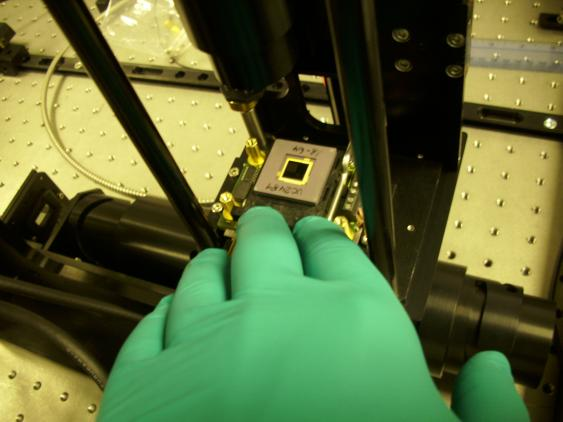
\includegraphics[width=7cm]{mma-plain}
%   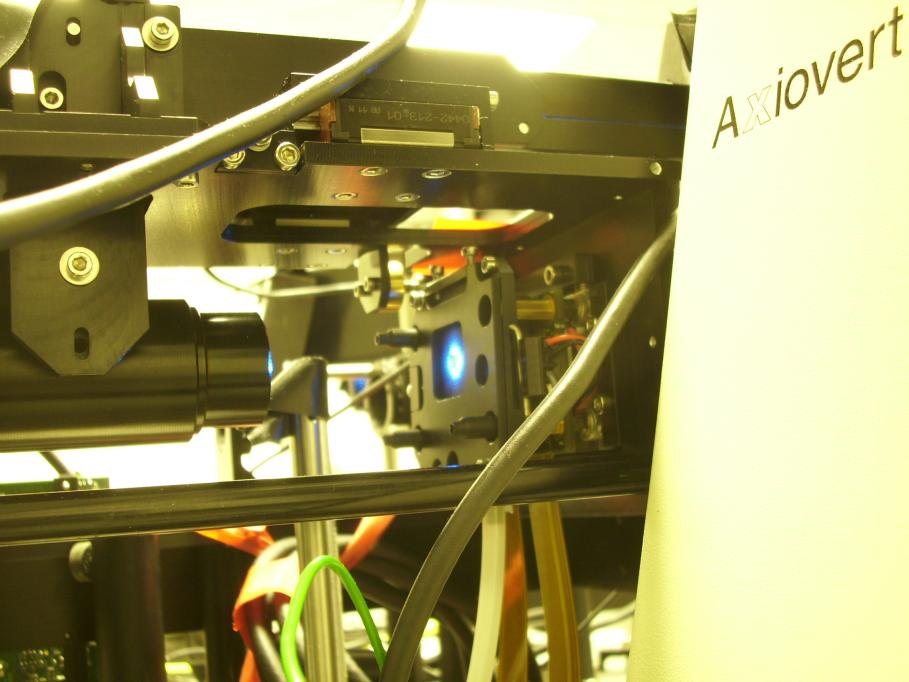
\includegraphics[width=7cm]{mma-ill}
%   \caption{{\bf left:} Micro mirror array chip during installation of
%     the optics. {\bf right:}~Illuminated micro mirror array in the
%     aligned system.}
%   \label{fig:mma-closeup}
% \end{figure}


\section{Mapping between pixels of the focal plane SLM and camera pixels}
\label{sec:map}
A basic prerequisite for measurement with our system is that the
mapping between SLM and camera pixels is known. Only then, the sample
can be irradiated as planned. To measure the mapping, I use a
fluorescent plane sample placed at the focal plane of the objective,
turn on individual pixels at position $\r^d$ of the focal plane SLM
and acquire camera images, which have bright spots centered on a
camera coordinate $\r^c$.

The fluorescent plane is attached directly to the underside of the
cover slip, ensuring good image quality and no (or negligibly small)
distortion.
\subsection{The rigid transform}
In our experiments, the following transformation with four degrees of
freedom (scaling $s$, rotation angle $\phi$, translation vector $\vect
t=(t_x,t_y)^T$) has proved particularly advantageous:
\begin{align}
  \label{eq:rigid}
  \r^d&=s \textrm{R}_\phi \r^c + \vect t\\
  \textrm{R}_\phi&=\begin{pmatrix}
  \cos\phi & q\sin\phi \\
  -\sin\phi & q\cos\phi \\ 
  \end{pmatrix}
\end{align}
where $\r^d=(r^d_x,r^d_y)^T$ is a point on the display,
$\r^c=(r^c_x,r^c_y)^T$ is a point on the camera and $R_\phi$ is a
rotation matrix. The value of $q$ depends on the arrangement of
mirrors in the beam path. The parameter $q$ is $-1$, if there is a
single axis reflection and it is $+1$ if there is no reflection.
\begin{figure}[!hbt]
  \centering
  \svginput{1}{calib-align}
  \caption{Given $n\ge 4$ camera images of a display showing one
    point.  It is possible to calculate the parameters of the rigid
    transform parameters scaling $s$, rotation angle $\phi$,
    translation vector $\vect t$.}
  \label{fig:calib-align}
\end{figure}

Alternatively, in the beginning we experimented with an affine
transformation. This transform is over-determined, as it includes two
additional degrees of freedom for shear and anisotropic scaling, which
are negligible in our system. Therefore it is difficult to assess the
quality of the calculated affine transform parameters.

With the rigid transform in equation (\ref{eq:rigid}), our system can,
however, be modeled very well: The camera is connected to a flange on
the microscope body and can be easily rotated. So when the camera is
moved, ideally, only the rotation angle $\phi$ needs to be
recalibrated. Similarly, the focal length setting of the illumination
tubelens $\textrm{TL}_\textrm{ill}$ mainly affects the scale $s$.
\subsubsection{Computational parameter estimation}
Having measured a set of $n\ge 4$ tuples $(\r^c_i,\r^d_i)$ of camera
and SLM coordinates, the four rigid transform parameters can be
obtained by minimizing the error $\mathcal{Q}$:
\begin{align}
 \mathcal{Q}= \sum_i^n \abs{s \textrm{R}_\phi \r^c_i+\vect t -\r^d_i}^2 \label{eq:rigid-sum}
\end{align}
There are good algorithms to solve this type of least squares problem.
In appendix \ref{sec:map_maxima} I show the source code for the
computer algebra system Maxima % FIXME stephan doesn't like the style
                               % of the reference
\citep{Maxima.sourceforge.net2013}. With ``Maxima'' the implementation
is particularly concise because it transparently calculates all the
necessary derivatives symbolically.

% In addition Maxima can easily be
% integrated in my real-time system.
% not really true for windows
\subsection{Experimental example and image processing}
Now I will show example images to describe the data collection for
measuring the transformation between camera pixels and focal plane
SLM.

For \cma{sample preparation} good results it is useful to have a
fluorescent plane sample that is homogeneous and without empty
(non-fluorescent) holes. I succeeded in making particularly thin and
uniform fluorescent planes with fluorescent beads. I prepared the
sample by drying an undiluted suspension of sub-diffraction,
fluorescent latex beads on a cover slip. This results in expanded areas
with uniform mono-, double- or multi-layers (see
\figref{fig:rigid-pics}).

It \cma{maximize field} is also advantageous if as large an area of
the focal plane SLM as possible is taken into account for the
estimation of the transform's parameters. Therefore I opened the two
diaphragms B0 and B1 (see \figref{fig:memi-real}) completely for the
calibration measurements.  I also kept the mirrors of the pupil plane
SLM undeflected to ensure maximum irradiance in the sample.

For \cma{scanning SLM pixel grid} the calibration I usually do not
only enable individual SLM pixels as this would give very dim images
with \unit[20]{ms} integration time. Instead, I enable pixels in a
circular area around the centre. This results in images as depicted in
\figref{fig:rigid-pics}~right. I acquired 100 such camera images while
moving the circular mask on the focal plane SLM over a $10\times 10$
grid (a disk of 24 focal plane SLM pixels diameter at the positions
$\r^d_{i+j}=(400+50i,500+50j)\ \forall i,j\in [0,99]$). Accidentally a
number of these points fell outside of the illuminated area and were
excluded from further processing.

In Appendix \ref{sec:matlab-spots} I show Matlab code (using the
DIPimage toolbox, \cite{dipimage}) to determine the position of the
bright spot in each camera image. Since the size of the illuminated
areas in the sample is bigger than the diffraction limit and
inhomogeneities of the fluorescent layer therefore will be visible in
the image, the image data must be corrected by dividing the pixel
values by the data of a uniformly illuminated image of the identical
region after background subtraction. Otherwise, sample non-uniformities would bias the results of
the localization algorithm.


\comment{
\jpginput{}{o102}{}
\jpginput{}{o035}{}
}

\begin{figure}[!hbt]
  \centering
  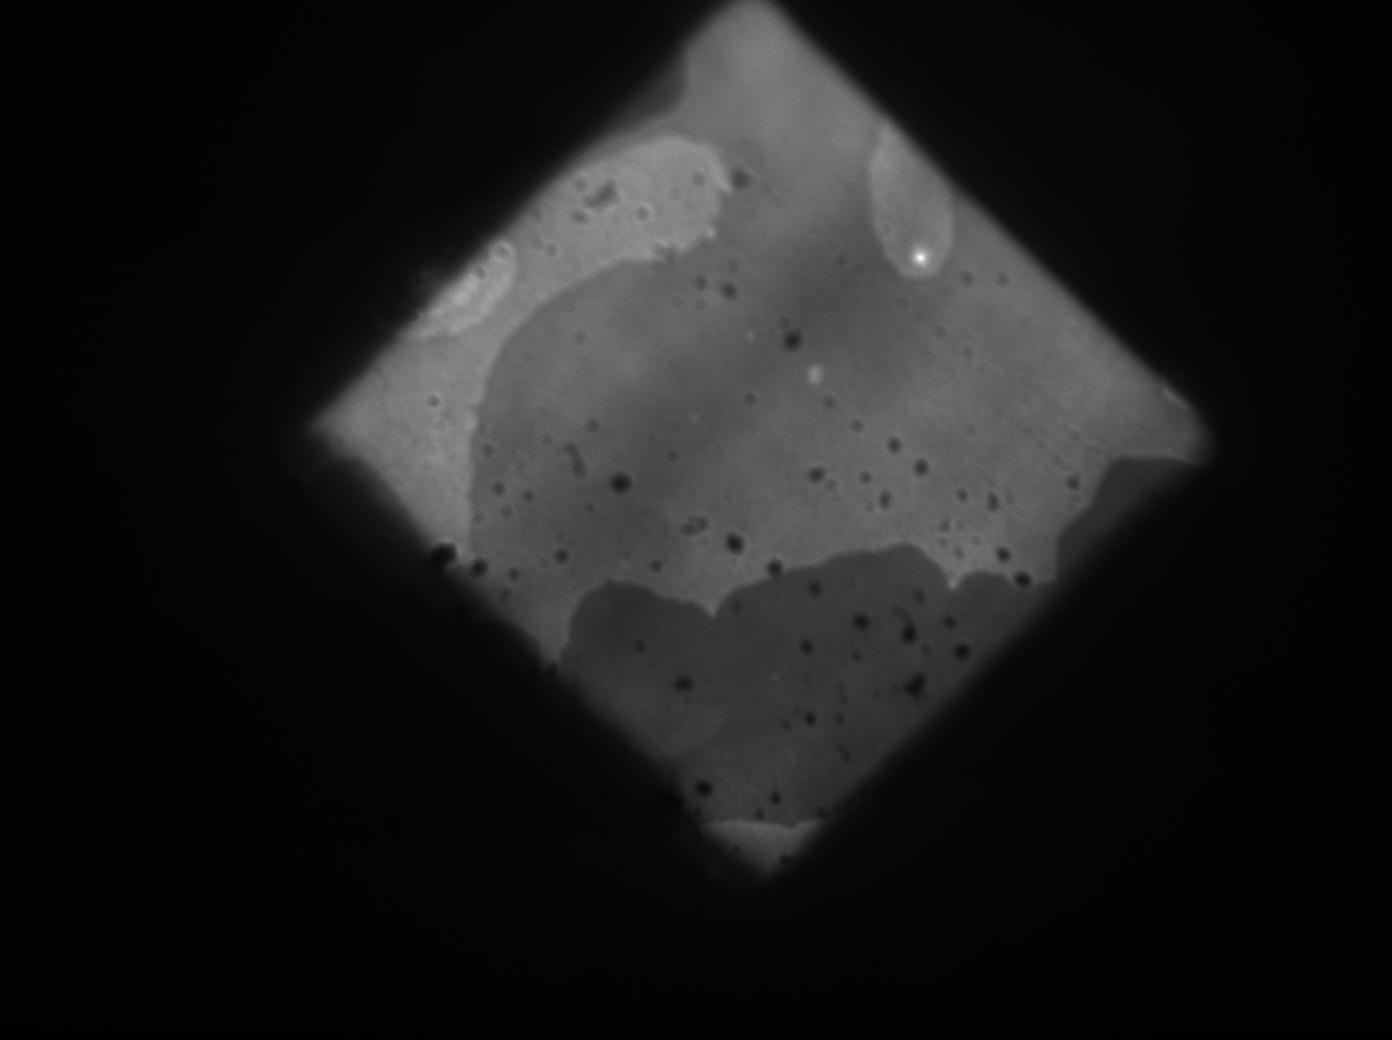
\includegraphics[width=4cm]{o102}\quad
  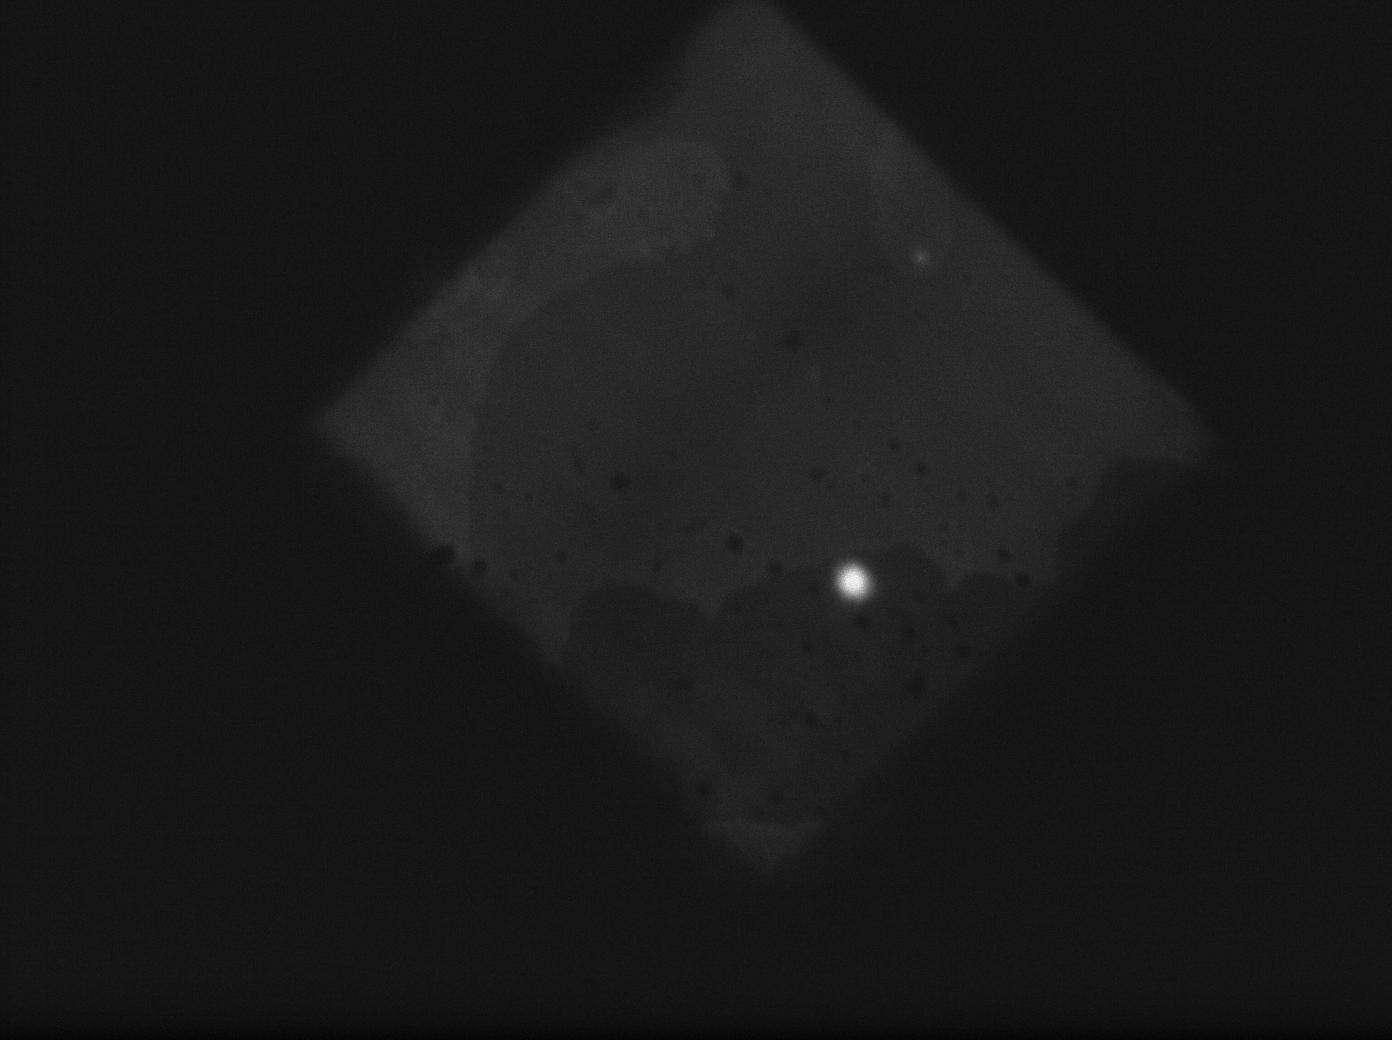
\includegraphics[width=4cm]{o035}
  \caption{{\bf left:} Uniformly illuminated fluorescent plane (mono
    and double layer of yellow beads with \unit[110]{nm} diameter,
    excited with \unit[473]{nm} laser in a $63\times$ objective with $\textrm{NA}=1.47$). {\bf
      right:} Image with the the focal plane SLM displaying a disk
    with 24 pixels diameter (corresponding to $\unit[2.4]{\mu m}$ in
    the sample) centred at focal plane SLM position $\r^d = (550,750)$.}
  \label{fig:rigid-pics}
\end{figure}

% i believe the TL_ill is set to r_MMA=3.84mm in BFP 
% f_TLill = 352 mm
% mag_real = mag / f_zeiss * f_TLill 
% pixel-pitch-lcos / mag_real
% one pixel is: 13.62 / 63 * 164.5 / 352 = 101nm


\begin{figure}[!hbt]
  \centering
  \pdfinput{10cm}{rigid-compare}
  \caption{Red ``$+$'' signs indicate where the spots that were
    localized in the camera images end up after a rigid
    transform. There is sufficient agreement with the original
    display positions.}
  \label{fig:rigid-compare}
\end{figure}

\figref{fig:rigid-compare} shows how well the transformed camera
coordinates ($\r^c$, indicated by '$+$' signs) superimpose with the
coordinates of the focal plane SLM pixel grid.


\figref{fig:screen_lcos-calib}~left depicts a pattern of discs that
was displayed on the focal plane SLM and the right figure shows a
superposition of the camera image and the outline of the circles.

\jpginput{7cm}{screen_lcos-calib}{Example of a rigid transform between
  focal plane SLM and camera. {\bf left:} Mask that is displayed on
  the SLM. {\bf right:} Camera image of fluorescent plane illuminated
  by mask. The orange outlines indicate the borders of the original
  pattern. The transformation between the coordinates fits very well
  and the illumination mask exactly covers the image, i.e.\ it is
  possible to selectively illuminate even small structures using the
  focal plane SLM.}

\subsection{Conclusion on the mapping transformation}
I have shown the simplest possible transformation to map between the
pixel grid of the camera and the focal plane SLM.

For this I have implemented a calibration routine using a computer
algebra system which would allow for more complicated transformations,
e.g.\ considering image distortion. However, my experiments have shown
that the simple transform is sufficient for our requirements and the
field of view, that the current illumination system supports.

The results of a calibration with this particular transformation can
be easily inverted. Furthermore, the interpretation of the parameters
and their fitting errors is obvious and simple.  In particular, the
fitted transform parameters scaling $s$, rotation $\phi$ and
translation $\vect t$ can be used directly in OpenGL to transform
vector primitives in and elegant way and with negligible computational
effort. I give example code in Appendix \ref{sec:map_opengl}.

\section{Optical sectioning by structured illumination}
\begin{summary}
  As mentioned in section \ref{sec:sectioning-intro} on page
  \pageref{sec:sectioning-intro}, a uniform signal of background
  fluorescence is inevitable in widefield microscopy. Here, I explain
  how in-focus and out-of-focus information can be separated by
  structured illumination.
\end{summary}
In order to provide maximum imaging speeds with our system, I
investigated techniques to obtain optically sectioned images with as
few exposures per slice as possible. Illuminating with a sinusoidal
grating has proved to be particularly advantageous because then the
necessary image processing can be expressed elegantly with linear
operations in Fourier space. Using the HiLo method \citep{Mertz2010},
already two acquisitions allow to calculate an optical section.

When a sinusoidal grating is imaged into the focal plane of a
microscope objective using incoherent light then the three-dimensional
light distribution in the sample has the $xz-$cross section shown in
\figref{fig:hilo-sec-Illum2}~left.  I generated this image by a
convolution of a sinusoidal transmission grating with the
three-dimensional point spread function of a $63\times$ oil ($n=1.52$)
immersion lens and $\textrm{NA}=1.4$.  The Matlab/DIPimage source code
that I used to generate the images in this section is listed in
appendix \ref{sec:sectioning} on page \pageref{sec:sectioning}.

For optical sectioning the essential effect that allows separation of
in-focus and out-of-focus light is that according to
\figref{fig:hilo-sec-Illum2} an in-focus fluorophore at point (a)
experiences a change in excitation intensity when the grating phase is
shifted. An out-of-focus fluorophore at point (b), however, is always
exposed to equal amounts of excitation light. There are many
possibilities to determine the degree of modulation in the acquired
images. Three of them I will introduce now.

\begin{figure}[htbp]
  \centering
  \svginput{1}{hilo-sec-Illum2} 
  \caption{{\bf left:} Light distribution in the sample for a
    $63\times$ objective with $NA=1.4$ and immersion index $n=1.52$
    using a grating pattern and incoherent illumination of wavelength
    $\lambda_0=\unit[500]{nm}$. {\bf right:} Cross-section of the
    in-focus optical transfer function (OTF) of this objective and
    spatial frequency spectrum of the in-focus light distribution.}
  \label{fig:hilo-sec-Illum2}
\end{figure}

For the simplest algorithm \citep{Benedetti1997} one assumes that the
in-focus information is responsible for the majority of the signal.
One can recover an approximation of the in-focus information by
calculating the maximum of a pixel value in the images $I_n$. Where
$n=1,\ldots,N$ denotes the phase of the pattern in each image.  The
out-of-focus background remains the same in each pixel of the raw
images and can be approximated by the minimum of each pixel value:
\begin{align} \label{eq:Iminmax}
  I_\textrm{max-min}(x,y) = \max_{n=1\ldots N}(I_n(x,y))- \min_{n=1\ldots N}(I_n(x,y))
\end{align}
However, this method has the disadvantage that the noise of the
reconstructed image does not decrease with an increasing number of
acquisitions $N$.  Another method, which is related to homodyne
detection \citep{Neil1997}, allows the separation of the modulated
signal if at least three raw images are available:
\begin{align} \label{eq:Ihomodyne}
  I_\textrm{homodyne}(x,y) = \left| \sum_{n=1\ldots N} I_n(x,y)\ e^{2\pi i n/N}\right|,\ \textrm{and}\ N\ge 3
\end{align}
In particular, with this approach each acquisition contributes to the
reconstructed optical section, resulting in a better noise performance
than the 'max-min' method.  In \figref{fig:hilo-sec-comparison}~c) and
d) I compared these reconstruction methods for $N=4$ using a simulated
fluorophore distribution as depicted in
\figref{fig:hilo-sec-comparison}~a).  In the simulated widefield image
\figref{fig:hilo-sec-comparison}~b) the intensity in the points 1 and
2 is similar, while the results of the sectioning algorithms in c), d)
and e) reject significant amounts of out-of-focus light in point 2.
\begin{figure}[htbp]
  \centering
  \svginput{1}{hilo-sec-comparison} 
  \caption{{\bf a)} Distribution of fluorophores for the simulations
    in this section. Two rectangles and a line intersecting a hollow
    sphere shell. {\bf b)} Widefield image in the slice with
    rectangle~1. {\bf c,d,e)} Optical sections of this slice using
    three different methods.  The brightest points of the raw images
    were set to contain 60000 photons and their photon shot noise was
    included in these simulations. The scalebars correspond to a
    wavelength of $\lambda_0=\unit[500]{nm}$.}
  \label{fig:hilo-sec-comparison}
\end{figure}

The reconstruction methods can all separate the rectangle from
background fluorescence. The simple 'max-min' method, however, causes
artifacts in the reconstruction. The spurious stripes would only
disappear if significantly more images were recorded. The homodyne
method gives a very good result but requires at least three images (I
used four to obtain \figref{fig:hilo-sec-comparison}~d).

In contrast, the HiLo method requires only two acquisitions (and I
used only two for \figref{fig:hilo-sec-comparison}~e). I will now
describe my version of the algorithm. The HiLo method was originally
developed for speckle illumination
\citep{Ventalon2005,Ventalon2007,Lim2011} but has also been used for
structured illumination with grating patterns
\citep{Bozinovic2008a,Mertz2010}.

Assuming the grating varies in the $x-$direction then the information
in the two raw images can be expressed as a superposition of modulated
in-focus information $I_\textrm{in}$ and out-of-focus information
$I_\textrm{out}$ that is the same in all raw images \citep{Mertz2010}:
\begin{align}
  I_n(x) = \left(1+m\sin(k_g x + n\pi)\right) I_\textrm{in}(x) + I_\textrm{out}(x),\
  \textrm{with}\ n=0,1
\end{align}
Here, $m$ is the modulation contrast and $k_g$ the spatial frequency
of the excitation pattern. For HiLo, the two raw images are combined
to form two new images:
\begin{align}
  I_\textrm{wf}(x) &= I_0(x)+I_1(x) = 2\left(I_\textrm{in} + I_\textrm{out}(x)\right) \\ 
  I_\textrm{demod}(x) &= I_0(x)-I_1(x) = 2 m \sin(k_g x) I_\textrm{in}  
\end{align}
%i0:(1+m*sin(x))*a+b;
%i1:(1+m*sin(x+%pi))*a+b;
%expand(i0+i1);
%expand(i0-i1)
The sum of the raw images corresponds to a widefield image with
uniform illumination, containing sectioned sample information only for
higher spatial frequencies (see \figref{fig:missing-cone} on page
\pageref{fig:missing-cone}). The image $I_\textrm{demod}$ allows
extraction of in-focus information for low spatial frequencies of the
fluorophore distribution. For HiLo, in-focus information from
different parts of the spatial frequency spectra of the images
$I_\textrm{wf}$ and $I_\textrm{demod}$ are combined to form the new
image $I_\textrm{hilo}(x)$:
\begin{align}
  I_\textrm{hilo}(x) = \eta\ \textrm{HP}(I_\textrm{wf}(x)) + \textrm{LP}\left(\textrm{FT}^{-1}\left[\frac{\widetilde I_\textrm{demod}(k-k_g)}{\textrm{OTF}(k)}\right](x)\right)
\end{align}
With the low-pass filter $\textrm{LP}$, whose cutoff frequency is
quite small, so that other orders of the spatial frequency spectrum of
$I_\textrm{demod}$ do not contribute to the signal (see
\figref{fig:hilo-method-description}~e).  \textrm{HP} is a the
complementary high-pass filter and the factor $\eta$ is introduced to
compensate for the modulation contrast $m$.  I divide by the optical
transfer function (see \figref{fig:hilo-sec-Illum2}) in order to
re-weight the sample information surrounding the first order in
$I_\textrm{demod}$. This is necessary because sample information on
different sides of the order were filtered differently by the optical
transfer function. Both $\eta$ and $k_g$ must be determined for each
experiment.  The algorithm in \citet{Mertz2010} does not require to
specify $k_g$ but their algorithm is non-linear and therefore gives
biased results in the presence of photon shot noise.
\begin{figure}[htbp]
  \centering
  \svginput{1}{hilo-method-description} 
  \caption{Application of my HiLo algorithm variant to a slice in the
    simulated fluorophore distribution from
    \figref{fig:hilo-sec-comparison}~a.}
  \label{fig:hilo-method-description}
\end{figure}

\subsection{Discussion and outlook on optical sectioning}
In this section, I have given an overview of different methods for
optical sectioning. In particular, I described a variant of the HiLo
reconstruction algorithm which requires only two exposures per slice
and is optimized for application in our instrument.

A thorough comparison of different algorithms in the presence of noise
is still pending. Furthermore, it would be helpful to examine which
projected grating frequencies will give the best sectioning
results. In the examples, which were shown here, a grating pattern of
high spatial frequency with the first order at $\nu_x\approx 1.3
\textrm{NA}/\lambda_0$ (see orange graph in
\figref{fig:hilo-sec-Illum2}~right) was used.  The best $z-$resolution
would be expected for $\nu_x= 1 \textrm{NA}/\lambda_0$ since there,
the support along $z$ of the three-dimensional optical transfer
function is widest (see \figref{fig:missing-cone}), with smaller
spatial frequencies the modulation contrast $m$ increases but so does
the overlap with adjacent orders.  The source code in appendix
\ref{sec:sectioning} should be a good starting point to investigate
these questions.

%%% Local Variables: 
%%% mode: latex
%%% TeX-master: "kielhorn_memi"
%%% eval: (reftex-mode)
%%% eval: (flyspell-mode)
%%% End: 
